\chapter{Performance Degradation}
\chapterauthor{Andrea Spinelli - Giacomo Amerio}

\section{Evaluation Metric: AUC}

We used the \textbf{Area under the Curve} (\textbf{AUC}) to evaluate model performance. The AUC measures the performance of a classification model by calculating the area under the ROC curve, which plots the true positive rate against the false positive rate. The AUC ranges from 0 to 1, where 0 indicates no predictive power and 1 indicates perfect predictive power.

Because the AUC focuses on how well the model ranks positive instances above negative ones, it is generally robust to shifts in the data distribution: if a positive and a negative example are chosen at random, the model should consistently rank the positive example higher than the negative one. 

\section{Models}

As metioned in the first chapter, simple covariate shift can lead to serious degradations in model performance. In this chapter, we will analyze how different statistical learning models' performances are affected by covariate shift. 

We evaluated a diverse set of models, ranging from simple linear classifiers to more sophisticated ensemble methods, to comprehensively assess their robustness under covariate shift conditions:

\begin{itemize}
    \item \textbf{Logistic Regression}: A linear classifier that serves as a baseline model;
    \item \textbf{Decision Tree}: A non-linear model that creates a tree-like structure of decision rules;
    \item \textbf{Generalized Additive Model (GAM)}: A flexible statistical model that combines the interpretability of linear models with the ability to capture non-linear relationships;
    \item \textbf{Random Forest}: An ensemble learning method that builds multiple decision trees and averages their predictions to improve performance;
    \item \textbf{Gradient Boosted Trees}: An ensemble learning method that creates sequential decision trees to iteratively correct prediction errors. Each tree focuses on the residuals from previous predictions, with optimized step sizes to minimize the overall loss function using gradient descent;
    \item \textbf{eXtreme Gradient Boosting (XGBoost)}: A highly optimized implementation of gradient boosting machines known for its efficiency and performance.
\end{itemize}

Each model was selected for its unique characteristics and widespread use in practical applications, providing a comprehensive view of how different learning approaches handle distribution shifts.

\section{Results}

We firstly evaluated the performance of each vanilla model on the aforementioned statistical mixtures of original and shifted test data. 

\begin{figure}[H]
    \centering
    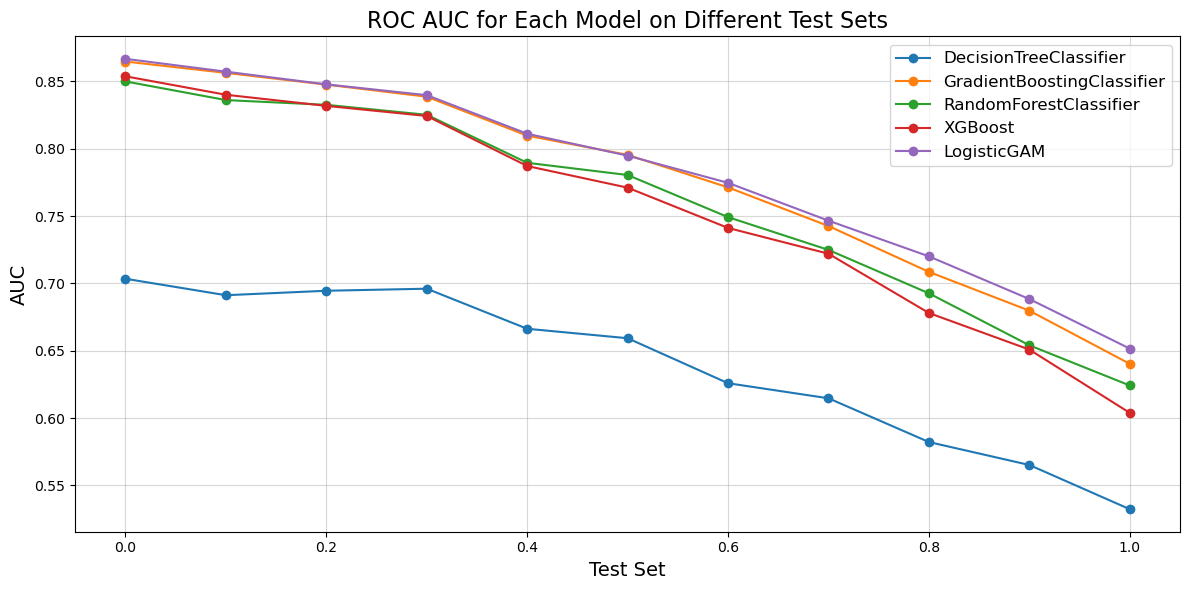
\includegraphics[width=0.8\textwidth]{assets/vanilla.png} 
    \caption{\textbf{Performance comparison of vanilla models under covariate shift.} The AUC scores of the models are plotted against the mixing probability $p$, which represents the proportion of shifted data in the test set.}
    \label{fig:vanilla-models-perf}
\end{figure}

As we can see from the plot, at low levels of mixed data, the models can still perform realatively well. However, as the proportion of mixed data increases, the performance of the models degrades significantly. The decision tree model is the most sensitive to covariate shift, while the GAM model is the most robust.

Given these preliminary results, we proceeded with hyperparameter optimization to potentially enhance model performance.

\subsubsection{Fine Tuning}

The best choice for hyperparameters in these models might be different depending on the dataset. In order to find the hyperparameters that best fit the data, we performed a hyperparameter tuning using the \plaintt{GridSearchCV} function from the \plaintt{scikit-learn} library, which performs a cross-validation (k=5) to select the best hyperparameters for each model, but only using the training set.
\begin{figure}[H]
    \centering
    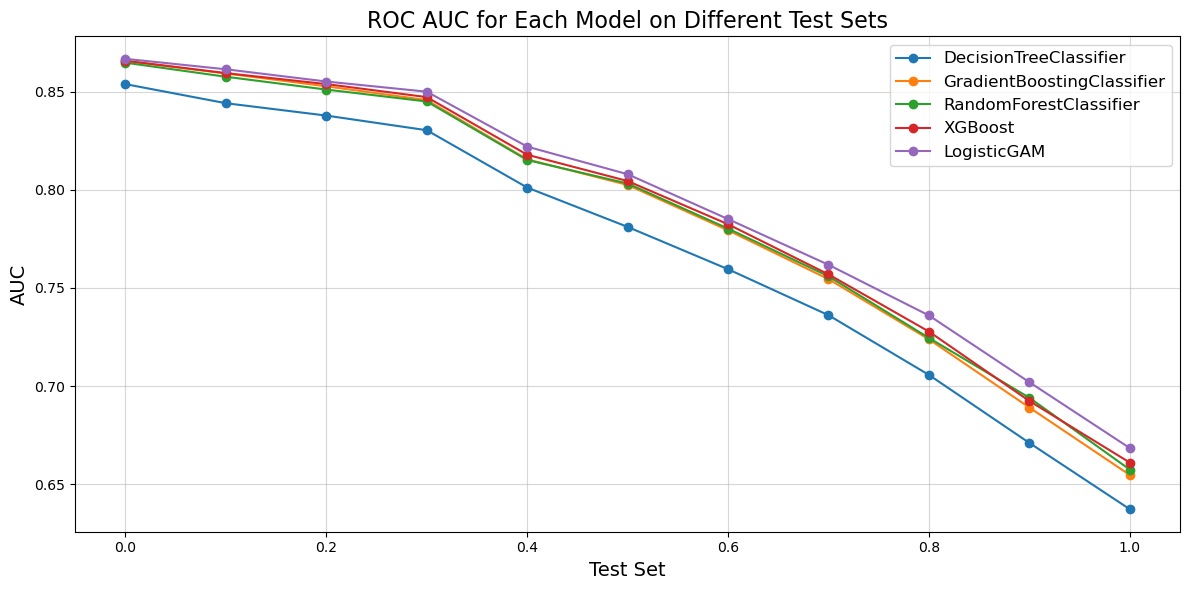
\includegraphics[width=0.8\textwidth]{assets/tuned.png} 
    \caption{\textbf{Performance comparison of fine tuned models under covariate shift.}}
    \label{fig:tuned-models-perf}
\end{figure}

As illustrated in \cref{fig:tuned-models-perf}, the fine-tuned models demonstrate improved performance relative to the baseline (vanilla) models. Notably, the decision tree model, which was previously the most affected by covariate shift, now performs nearly on par with the other models. Overall, all models—except for Logistic Regression—exhibit a marked improvement in performance. Among them, the XGBoost and Random Forest models consistently achieve the highest AUC scores. However, none of these models appears to outperform the others definitively, as they all exhibit similar behavior. It is important to note that the fine-tuning process is still ongoing.

